\section{Файловые диалоги и работа с файлами}

\textbf{Задание:} Создать таблицу Work. В другой файл вывести данные о рабочих, занимающих данную должность. (Вариант 14)

Вид окна представлен на рисунке \ref{fig:task8_form}.
\begin{figure}[H]
    \centering
    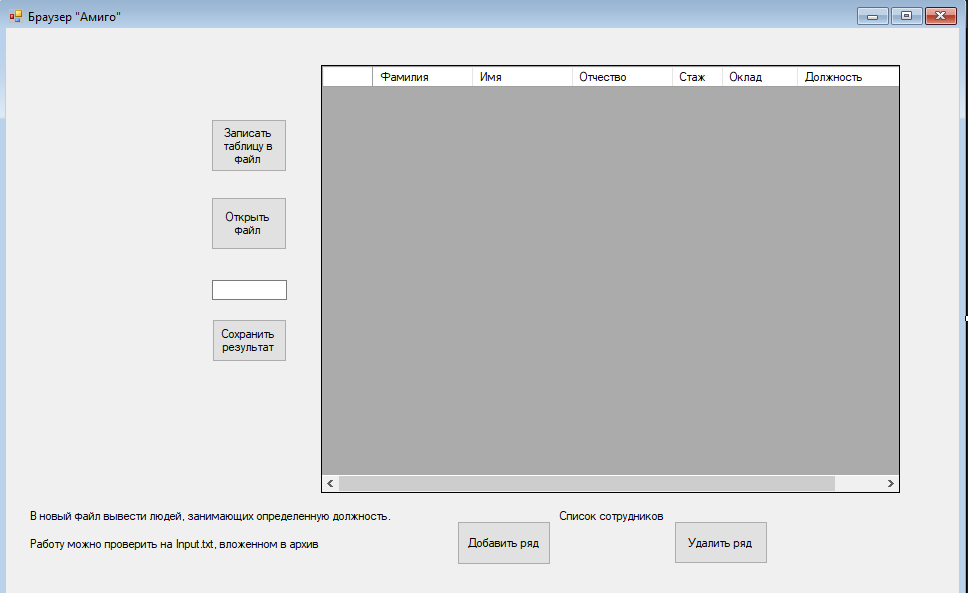
\includegraphics[scale=0.7]{task8/form.png}
    \caption{Внешний вид формы программы}
    \label{fig:task8_form}
\end{figure}
У элементов изменены значения некоторых атрибутов. 
Значения измененных атрибутов представлены в таблице \ref{table:params8}.
\begin{longtable}{|l|l|}
    Наименование атрибута & Значение\cr\hline
    \multicolumn{2}{|l|}{Для формы}\cr\hline
    \verb"Text" & \verb"Браузер "Амиго""\cr\hline
    \verb"FormBorderStyle" & \verb"FixedSingle"\cr\hline
    \verb"MaximizeBox" & \verb"False"\cr\hline
    \multicolumn{2}{|l|}{Для таблицы}\cr\hline
    \verb"(Name)" & \verb"gridResult"\cr\hline
    \multicolumn{2}{|l|}{Для кнопки записи в файл}\cr\hline
    \verb"(Name)" & \verb"SaveFileBtn"\cr\hline
    \multicolumn{2}{|l|}{Для кнопки открытия файла}\cr\hline
    \verb"(Name)" & \verb"OpenFileBtn"\cr\hline
    \multicolumn{2}{|l|}{Для кнопки сохранения результата}\cr\hline
    \verb"(Name)" & \verb"ResultBtn"\cr\hline
    \multicolumn{2}{|l|}{Для текстового поля должности}\cr\hline
    \verb"(Name)" & \verb"ResultTextBox"\cr\hline
    \multicolumn{2}{|l|}{Для обработчика ошибок}\cr\hline
    \verb"(Name)" & \verb"errorProvider1"\cr\hline

    \caption{Значения атрибутов элементов в приложении <<Работа с файлами>>}
    \label{table:params8}
\end{longtable}
Кроме того, это приложение содержит элементы \verb|openFileDialogue|
и \verb|saveFileDialogue|, реализующие открытие и сохранение файлов.

Работа с ними производится в кнопках. Ниже приведен пример работы
функции открытия файла:
\begin{minted}[fontsize=\footnotesize, breaklines=true, style=bw, linenos]{cpp}
private: System::Void OpenFileBtn_Click(System::Object^ sender, System::EventArgs^ e) {
	System::IO::Stream^ myStream;
	if (this->openFileDialog->ShowDialog() == System::Windows::Forms::DialogResult::OK) {
		CreateEmptyMatrix(gridResult, 1);
		if ((myStream = openFileDialog->OpenFile()) != nullptr) {
			System::IO::StreamReader^ sw = gcnew System::IO::StreamReader(myStream, System::Text::Encoding::
			GetEncoding(65001)); // UTF-8
			System::String^ s = "";
			int innerIdx = 0;
			while ((s = sw->ReadLine()) != nullptr && s != "") {
				gridResult->Rows->Add(1);
				int idx = 0;
				int current = 0;
				while (idx != s->Length) { 
					System::String^ currentWord = "";
					while (idx < s->Length && s[idx] != ' ') {
						currentWord += s[idx++];
					}
					if (idx < s->Length && s[idx] == ' ') ++idx;
					gridResult->Rows[innerIdx]->Cells[current++]->Value = currentWord;
					currentWord = "";
				}
				++innerIdx;
			}
		sw->Close();
		}
	}
}
\end{minted}

После запуска программы на экране появляется окно следующего вида (см. рисунок \ref{fig:exec8})
\begin{figure}[H]
    \centering
    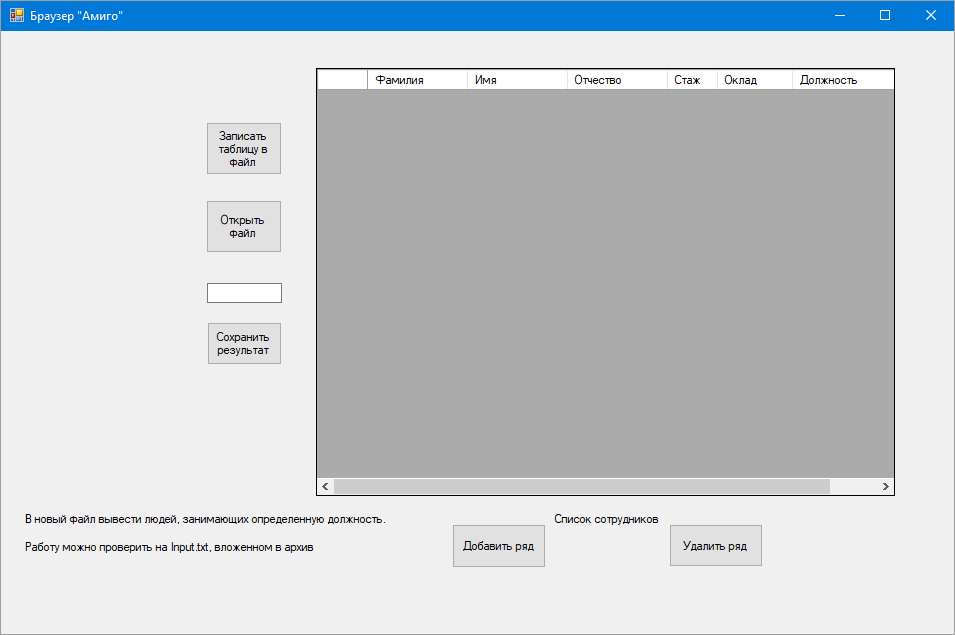
\includegraphics[scale=0.4]{task8/exec.png}
    \caption{Внешний вид окна приложения}
    \label{fig:exec8}
\end{figure}

После открытия файла состояние программы изменится на следующее (см. рисунок \ref{fig:openFile})
\begin{figure}[H]
    \centering
    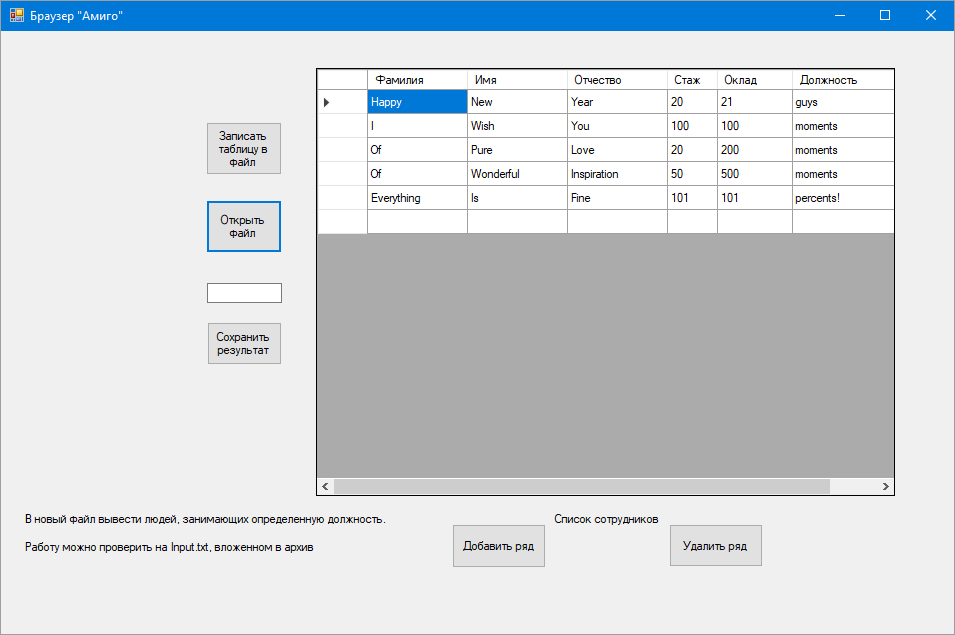
\includegraphics[scale=0.4]{task8/openFile.png}
    \caption{Состояние программы после открытия файла}
    \label{fig:openFile}
\end{figure}

Результатом работы программы является новый файл (см. рисунок \ref{fig:result8})
\begin{figure}[H]
    \centering
    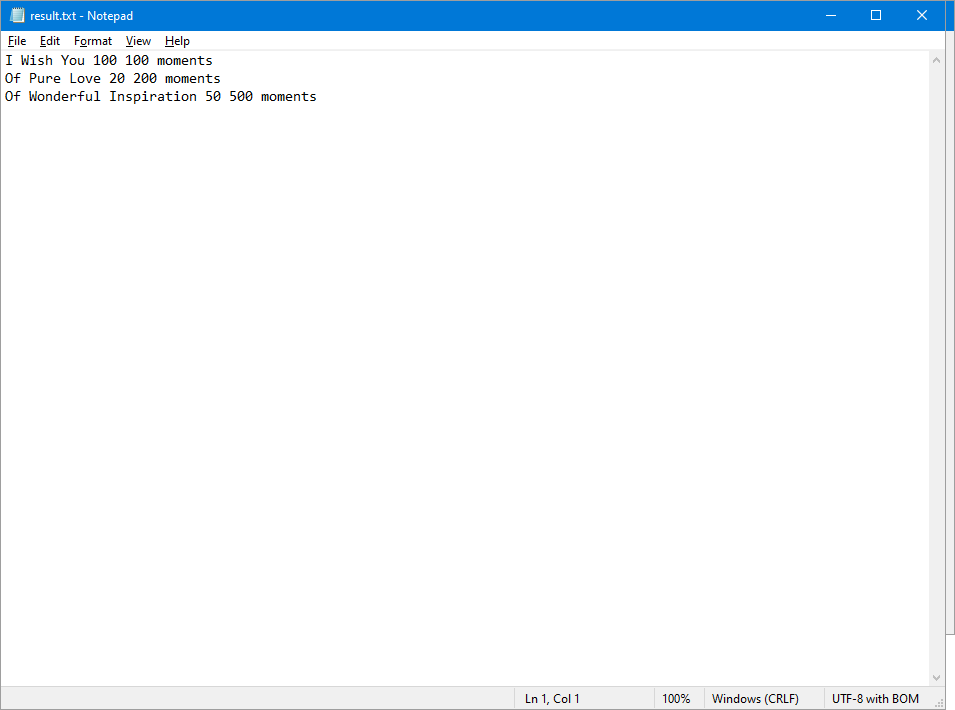
\includegraphics[scale=0.4]{task8/result.png}
    \caption{Результат работы программы}
    \label{fig:result8}
\end{figure}
Возникновение исключительных ситуаций ограничено интерфейсом, постановкой задачи
и программными средствами \verb|.NET framework|.

Полный код программы приведен в приложении \ref{app:repos}.

